\documentclass{jsarticle}
\oddsidemargin=-0.8cm
\topmargin=-2cm
\baselineskip=13pt
\textheight=55\baselineskip
\marginparsep=0.5in
\marginparwidth=0.5in
\textwidth=52zw
\usepackage{ascmac}
\usepackage{url}
\usepackage[dvipdfmx]{graphicx}
\usepackage[dvipdfmx]{color}
\usepackage{amsmath}
\usepackage{amssymb}
\usepackage{multicol}
\usepackage{bm}
\usepackage{enumerate}
\usepackage{listings}
\usepackage{fancybox}
\usepackage{framed}
\usepackage{subfigure}
\usepackage{ccaption}
\usepackage{color}
\makeatletter
\lstset{% 
language={C}, 
frame=trbl,% 
basicstyle={\small},% 
identifierstyle={\small},% 
commentstyle={\small\ttfamily},% 
keywordstyle={\small\bfseries},% 
ndkeywordstyle={\small},% 
stringstyle={\small\ttfamily}, 
tabsize=2,
breaklines=true, 
frame=none,
columns=[l]{fullflexible},% 
numbers=left,% 
xrightmargin=0zw,% 
xleftmargin=3zw,% 
numberstyle={\scriptsize},% 
stepnumber=1, 
numbersep=1zw,% 
backgroundcolor={\color[gray]{.90}},
} 
\makeatother

\newenvironment{problems}
{
  \renewcommand\labelenumi{\doublebox{\arabic{enumi}}}
  \begin{enumerate}
}{
  \end{enumerate}
  \renewcommand\labelenumi{\arabic{enumi}.}
}

\pagestyle{empty}	

\begin{document}
\title{基礎気象学講義 復習問題} % ここは毎回同じ
\author{第1回} %authorの代わりに第何回かを入れる
\date{大気概観} %内容を記載する
\maketitle

\section{問題}

    \begin{problems}
    \item 次の文章を読んで、後の問いに答えなさい。
        \begin{screen}
        大気圏の構造は気温によって特徴づけられ、気温が極大や極小になる高さを境に、次の通り大きく4つの層に分けられる。

            \begin{itemize}
            \item (A):地表から高さ約10kmまでの範囲を言い、平均的には(B)K/kmの気温減率で上空に行くほど気温が下がっていく。
            この層では、雲や雨と言った気象現象あるいは前線や低気圧と言った擾乱(じょうらん:気象学においては大気の定常状態からその流れが乱れることをさす用語。
            流れを乱すものであれば高気圧などもこれに該当するが、単にこの言葉を使った場合、多くは降水性のものを示す。)が起こる。
            この上端は(C)と呼ばれ、$_{(\mathrm{a})}$\underline{極に行くほど高く、年単位では冬よりも夏、日単位では夜よりも日中に高い傾向にある。}
            \item (D):(C)からおおよそ高さ50kmまでの範囲である。約20kmの高度までは気温が一定で、上に行くと気温が高くなり、50kmのところで最大となる。
            基本的には安定成層であり、(A)に対する蓋のような役割を果たす層であるが、ブリューワー・ドブソン循環と呼ばれる大規模な大気の運動や、準2年周期変動、突然昇温と言った物理的現象の起こる層でもある。
            また、オゾン層が存在するのもこの層で、紫外線の吸収などの役割を果たしている。近年、南極を中心に$_{(\mathrm{b})}$\underline{オゾンの濃度が薄くなっており、(E)と呼ばれる環境問題として知られている。}
            \item (F):高さ50kmから80kmほどの範囲である。高度に連れて気温が下がっていく。
            \item (G):(F)より上の範囲を言い、はっきりした上限はない。
            この部分は高度に連れて気温があがり、$_{(\mathrm{c})}$\underline{約400kmでは1000Kほどになる。}だが、この層での熱量は地表付近に比べてずっと小さい。これは、密度が小さいためである。
            また、ここでは分子が原子を経てイオンや電子に電離する層がある。これを(H)と呼び、電気伝導度が大きい状態にある。
            電離が特に集中している層を、下からD層・E層・F層と呼ぶ。$_{(\mathrm{d})}$\underline{この層の存在により、地球上では電波が遠くまで伝わる。}
            \end{itemize}
            \begin{flushright}
            (白木「新 百万人の天気教室」を元に作成)
            \end{flushright}
        \end{screen}

        \begin{enumerate}[(1)]
        \item 文中の空欄(A)〜(H)に当てはまる語句や数値を答えなさい。
        \item 下線部(a)のように、(C)が緯度や年単位・日単位で変動するのは何故か説明しなさい。
        \item 下線部(b)については、エアコン等の冷媒として使われたフロンガスが原因とされますが、実際にはそれ以外の物質も多くあり、いずれも触媒の役割を果たします。
              破壊はオゾンが酸素になることにより起きますが、その化学反応式を答えなさい。
        \item 下線部(c)に関連して、この高度では一般にやけどしないが、なぜか答えなさい。
        \item 下線部(d)について、この層がどのような役割を果たして電波が遠くまで伝わるのか、その理由を述べなさい。\\
        \end{enumerate}

    \item 地球を含む太陽系の惑星(全8つ)について、その大気組成から、大気の平均物質量を求めなさい。\\

    \item Atmospheric Soundingsのサイト(\url{http://weather.uwyo.edu/upperair/sounding.html})では、様々な地点の高層観測結果を取得できます。
        \begin{enumerate}[(1)]
        \item 国内の適当な地点について、何通りかの日時(春夏秋冬の昼夜がそれぞれカバーできるのが望ましい)の観測データを取得し、横軸を気温・縦軸を気圧の対数軸としたグラフを書きなさい。
            また、この内一つの日時について、同程度の経度で緯度が異なる北半球のいくつかの地点についても同じグラフを作成しなさい(こちらは国内でなくてよい)。
        \item グラフから各圏界面の高度(気圧)を求めなさい。
        \item 圏界面高度の変化や大気の層構造について、気づいた点を述べなさい。(気象庁サイトなどから当日の地上観測データ等を取得して合わせて考察しても構いません。)
        \end{enumerate}
\end{problems}

\section{答案}
\begin{problems}
% 以下に解答を作成してGit Push。
\item
        \begin{enumerate}[(1)]
        \item
        (A)対流圏
        (B)6.5
        (C)対流圏界面
        (D)成層圏
        (E)地球温暖化
        (F)中層圏
        (G)熱圏
        \item
        季節や昼夜があるため、対流圏の気温が変わるため。暑い日は上に押し上げられ、寒い日は下に押し下げられる。
        \item
        $2O_3 \rightarrow 3O_2$
        \item
        熱圏は分子密度が低いため、熱が伝わりにくいから。
        \item
        電離層で分子が電離しているから。
        \end{enumerate}

\item



\item
        \begin{enumerate}[(1)]
        \item
        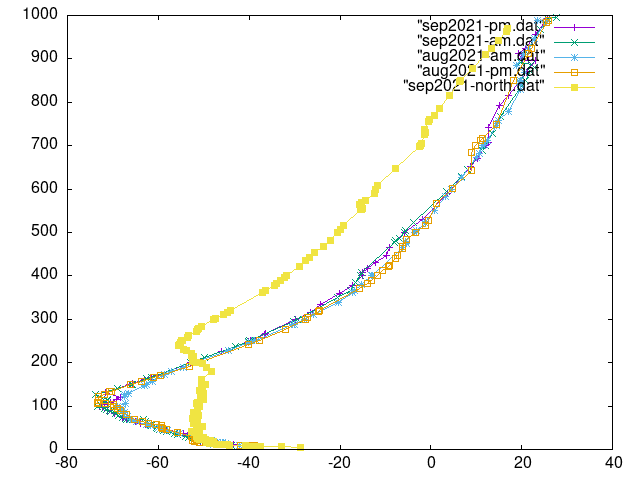
\includegraphics[width=3cm]{graph.png}
        \item
        (日本)
        対流圏界面:115.603
        残りはグラフから読み取れず。 \\
        (北半球のFort Nelson)
        対流圏界面:44.0093
        成層圏界面:185.092
        中間圏界面:244.051
        \item
        グラフから読み取るに、北に行けば行くほど、圏界面の高度は上がるのではないかと予測ができる。 \\
        また、日本のグラフを見ても、対流圏界面しか読み取ることができなかった。場所によって、層の厚さが違うのではないか?\\
        基礎気象学と比べたら、北半球のところは明らかに低すぎる。読み取りミスか、寒いため、低くなっているのではないかと予測できる
        \end{enumerate}

\end{problems}


\end{document}

